% Options for packages loaded elsewhere
\PassOptionsToPackage{unicode}{hyperref}
\PassOptionsToPackage{hyphens}{url}
%
\documentclass[
]{article}
\usepackage{lmodern}
\usepackage{amssymb,amsmath}
\usepackage{ifxetex,ifluatex}
\ifnum 0\ifxetex 1\fi\ifluatex 1\fi=0 % if pdftex
  \usepackage[T1]{fontenc}
  \usepackage[utf8]{inputenc}
  \usepackage{textcomp} % provide euro and other symbols
\else % if luatex or xetex
  \usepackage{unicode-math}
  \defaultfontfeatures{Scale=MatchLowercase}
  \defaultfontfeatures[\rmfamily]{Ligatures=TeX,Scale=1}
\fi
% Use upquote if available, for straight quotes in verbatim environments
\IfFileExists{upquote.sty}{\usepackage{upquote}}{}
\IfFileExists{microtype.sty}{% use microtype if available
  \usepackage[]{microtype}
  \UseMicrotypeSet[protrusion]{basicmath} % disable protrusion for tt fonts
}{}
\makeatletter
\@ifundefined{KOMAClassName}{% if non-KOMA class
  \IfFileExists{parskip.sty}{%
    \usepackage{parskip}
  }{% else
    \setlength{\parindent}{0pt}
    \setlength{\parskip}{6pt plus 2pt minus 1pt}}
}{% if KOMA class
  \KOMAoptions{parskip=half}}
\makeatother
\usepackage{xcolor}
\IfFileExists{xurl.sty}{\usepackage{xurl}}{} % add URL line breaks if available
\IfFileExists{bookmark.sty}{\usepackage{bookmark}}{\usepackage{hyperref}}
\hypersetup{
  hidelinks,
  pdfcreator={LaTeX via pandoc}}
\urlstyle{same} % disable monospaced font for URLs
\usepackage[margin=1in]{geometry}
\usepackage{graphicx}
\makeatletter
\def\maxwidth{\ifdim\Gin@nat@width>\linewidth\linewidth\else\Gin@nat@width\fi}
\def\maxheight{\ifdim\Gin@nat@height>\textheight\textheight\else\Gin@nat@height\fi}
\makeatother
% Scale images if necessary, so that they will not overflow the page
% margins by default, and it is still possible to overwrite the defaults
% using explicit options in \includegraphics[width, height, ...]{}
\setkeys{Gin}{width=\maxwidth,height=\maxheight,keepaspectratio}
% Set default figure placement to htbp
\makeatletter
\def\fps@figure{htbp}
\makeatother
\setlength{\emergencystretch}{3em} % prevent overfull lines
\providecommand{\tightlist}{%
  \setlength{\itemsep}{0pt}\setlength{\parskip}{0pt}}
\setcounter{secnumdepth}{-\maxdimen} % remove section numbering

\author{}
\date{\vspace{-2.5em}}

\begin{document}

\hypertarget{the-structure-of-scientific-writing}{%
\section{The Structure of Scientific
Writing}\label{the-structure-of-scientific-writing}}

\hypertarget{learning-objectives}{%
\subsection{Learning Objectives}\label{learning-objectives}}

\begin{enumerate}
\def\labelenumi{\arabic{enumi}.}
\item
  Understand the basic sections of scientific papers.
\item
  Develop a plan for how to build your paper.
\end{enumerate}

\hypertarget{how-science-is-made}{%
\subsection{How Science is Made}\label{how-science-is-made}}

There are millions of scientific papers in published journals and
thousands of university lab courses that require scientific papers in
some form. The vast majority have these sections:

\begin{itemize}
\tightlist
\item
  \emph{Title}
\item
  \emph{Abstract}
\item
  \emph{Introduction}
\item
  \emph{Methods}
\item
  \emph{Results}
\item
  \emph{Discussion}
\item
  \emph{References}
\item
  \emph{Tables}
\item
  \emph{Figures}
\end{itemize}

Later chapters of this book will discuss each of these in detail. In
this chapter, we briefly introduce each section and then provide a guide
for how to approach your writing project so that these rigid sections
become a fluid and interesting scientific story. The lecture for this
section is here:
\href{https://docs.google.com/presentation/d/1t8Ggc_xpu1eapc2UbTm8kGzCPWLQLi4AXnKyjM_4jKM/edit?usp=sharing}{Lecture
Link}

\hypertarget{title}{%
\subsection{Title}\label{title}}

\begin{itemize}
\tightlist
\item
  Short and descriptive
\end{itemize}

\hypertarget{abstract}{%
\subsection{Abstract}\label{abstract}}

\begin{itemize}
\tightlist
\item
  One or two sentences that introduce the topic.
\item
  One sentence that states your hypothesis.
\item
  One sentence that briefly states what you did for methods.
\item
  Two-three sentences of the \emph{main} results with some quantitative
  information as needed (but no p-values).
\item
  One or two sentences that summarize the main finding.
\end{itemize}

\hypertarget{introduction}{%
\subsection{Introduction}\label{introduction}}

\begin{itemize}
\tightlist
\item
  What big question are you going to answer for us?
\item
  Why is this question important?
\item
  Lots of references
\item
  4-5 paragraphs is usually plenty.
\end{itemize}

\hypertarget{methods}{%
\subsection{Methods}\label{methods}}

\begin{itemize}
\tightlist
\item
  What did you do to answer this important question?
\item
  How did you analyze your data?
\item
  Write what you did in a way that other people could repeat it.
\item
  Doesn't matter that your instructor knows what you did. It just
  matters that \emph{other scientists} could understand it.
\item
  Few references.
\item
  2-8 paragraphs is usually plenty.
\end{itemize}

\hypertarget{results}{%
\subsection{Results}\label{results}}

\begin{itemize}
\tightlist
\item
  Write what you discovered.
\item
  Clear and simple and quantitative.
\item
  Don't interpret anything. Just report the basic results.
\item
  Usually zero references here.
\item
  1-4 paragraphs is usually plenty.
\end{itemize}

\hypertarget{discussion}{%
\subsection{Discussion}\label{discussion}}

\begin{itemize}
\tightlist
\item
  Now you can interpret
\item
  \emph{The most important result of this study was\ldots{}}
\item
  Lots of references.
\item
  4-6 paragraphs is usually plenty.
\end{itemize}

\hypertarget{references}{%
\subsection{References}\label{references}}

\begin{itemize}
\tightlist
\item
  What is known and unknown?
\item
  Establishes trust between writer and reader.
\item
  Gives credit to other ideas.
\item
  Pick one format (there are lots of ways to write citations) and stick
  to it.
\end{itemize}

\hypertarget{tables}{%
\subsection{Tables}\label{tables}}

\begin{itemize}
\tightlist
\item
  Summary statistics or raw data
\end{itemize}

\hypertarget{figures}{%
\subsection{Figures}\label{figures}}

\begin{itemize}
\tightlist
\item
  Make the font readable
\item
  Make them as simple as possible
\item
  The reader should be able to guess what the figure axes will be based
  on the written sections above. No surprises.
\end{itemize}

\hypertarget{putting-it-all-together}{%
\section{Putting it all together}\label{putting-it-all-together}}

You are probably familiar with some or all of these sections of a
scientific paper. The next challenge is harder - finding a way to put
these sections together so that they result in an understandable and
perhaps even enjoyable thing to read. That is the hard part, and it's
why you're taking this class or reading this book. Here are some tips to
get you started.

\begin{enumerate}
\def\labelenumi{\arabic{enumi})}
\tightlist
\item
  \emph{Hourglass Structure}
\end{enumerate}

Think of your scientific paper as having a beginning that sets out the
broad ideas, a middle that has all of the technical details, and an end
that leaves you with a core take-home message. A common way to visualize
that is with an hourglass in which each each section of the paper moves
from top to bottom (Fig. 1). The narrower sections have technical
details that are relevant to your specific study. The broader sections
relate those details to broader ideas. Often it can be easier to write
the middle parts first.

\begin{figure}

\begin{figure}

\includegraphics[width=0.6\linewidth]{C:/Users/Jeff.Wesner/Documents/GitHub/Inquiry_Textbook/images/hourglass} \caption{The hourglass structure of a scientific paper. The width of the hourglass reflects the purpose of each secion. The overall paper leads the reader from a broad concept to specific methods and results. Then it tells the reader how those specific results have changed our understanding of the broader concept in the introduction.}\label{fig:unnamed-chunk-1}
\end{figure}

\end{figure}

\begin{enumerate}
\def\labelenumi{\arabic{enumi})}
\setcounter{enumi}{1}
\tightlist
\item
  \emph{Figures First}
\end{enumerate}

One of our favorite ways to start writing a paper is to not write at
all, but instead to work on the figures first. By figures, we mean the
plots (or charts or data visualizations, etc) that show your scientific
results.

Here's an example using a manuscript that one of us wrote
{[}@wesner\_forecasting\_2020{]}.

\begin{figure}
\begin{figure}
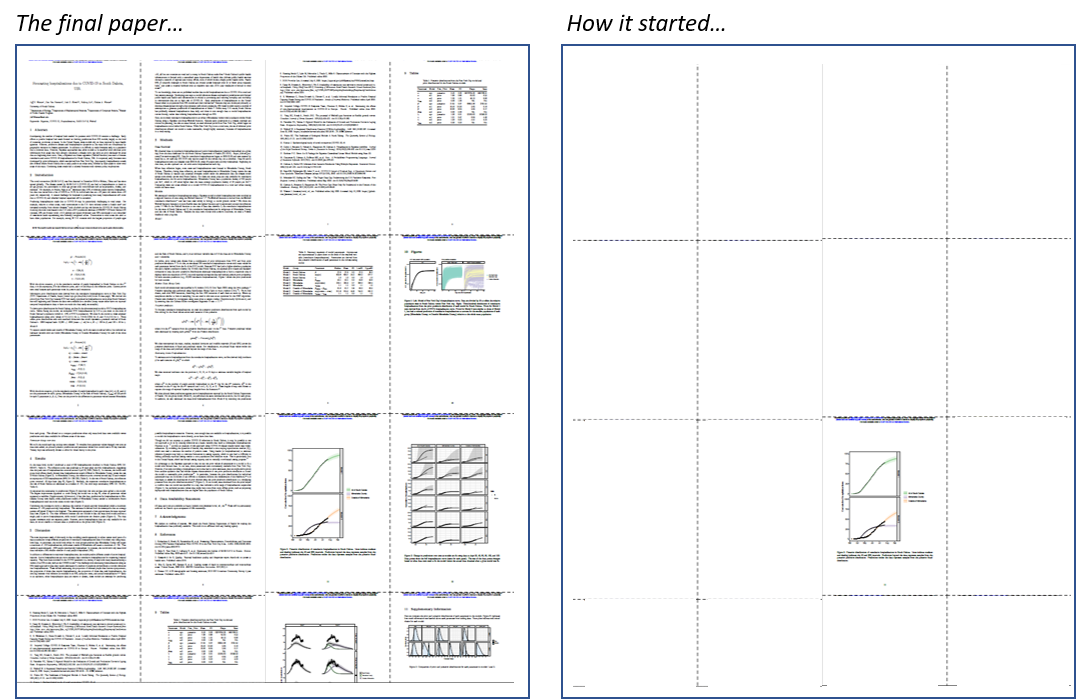
\includegraphics[width=1\linewidth]{C:/Users/Jeff.Wesner/Documents/GitHub/Inquiry_Textbook/images/covid_paper_all} \caption{The final paper for Wesner et al. 2020 had lots of technical details and broader context about COVID hospitalizations (left). But it started with only a single figure (right).}\label{fig:unnamed-chunk-2}
\end{figure}
\end{figure}

\begin{figure}
\begin{figure}
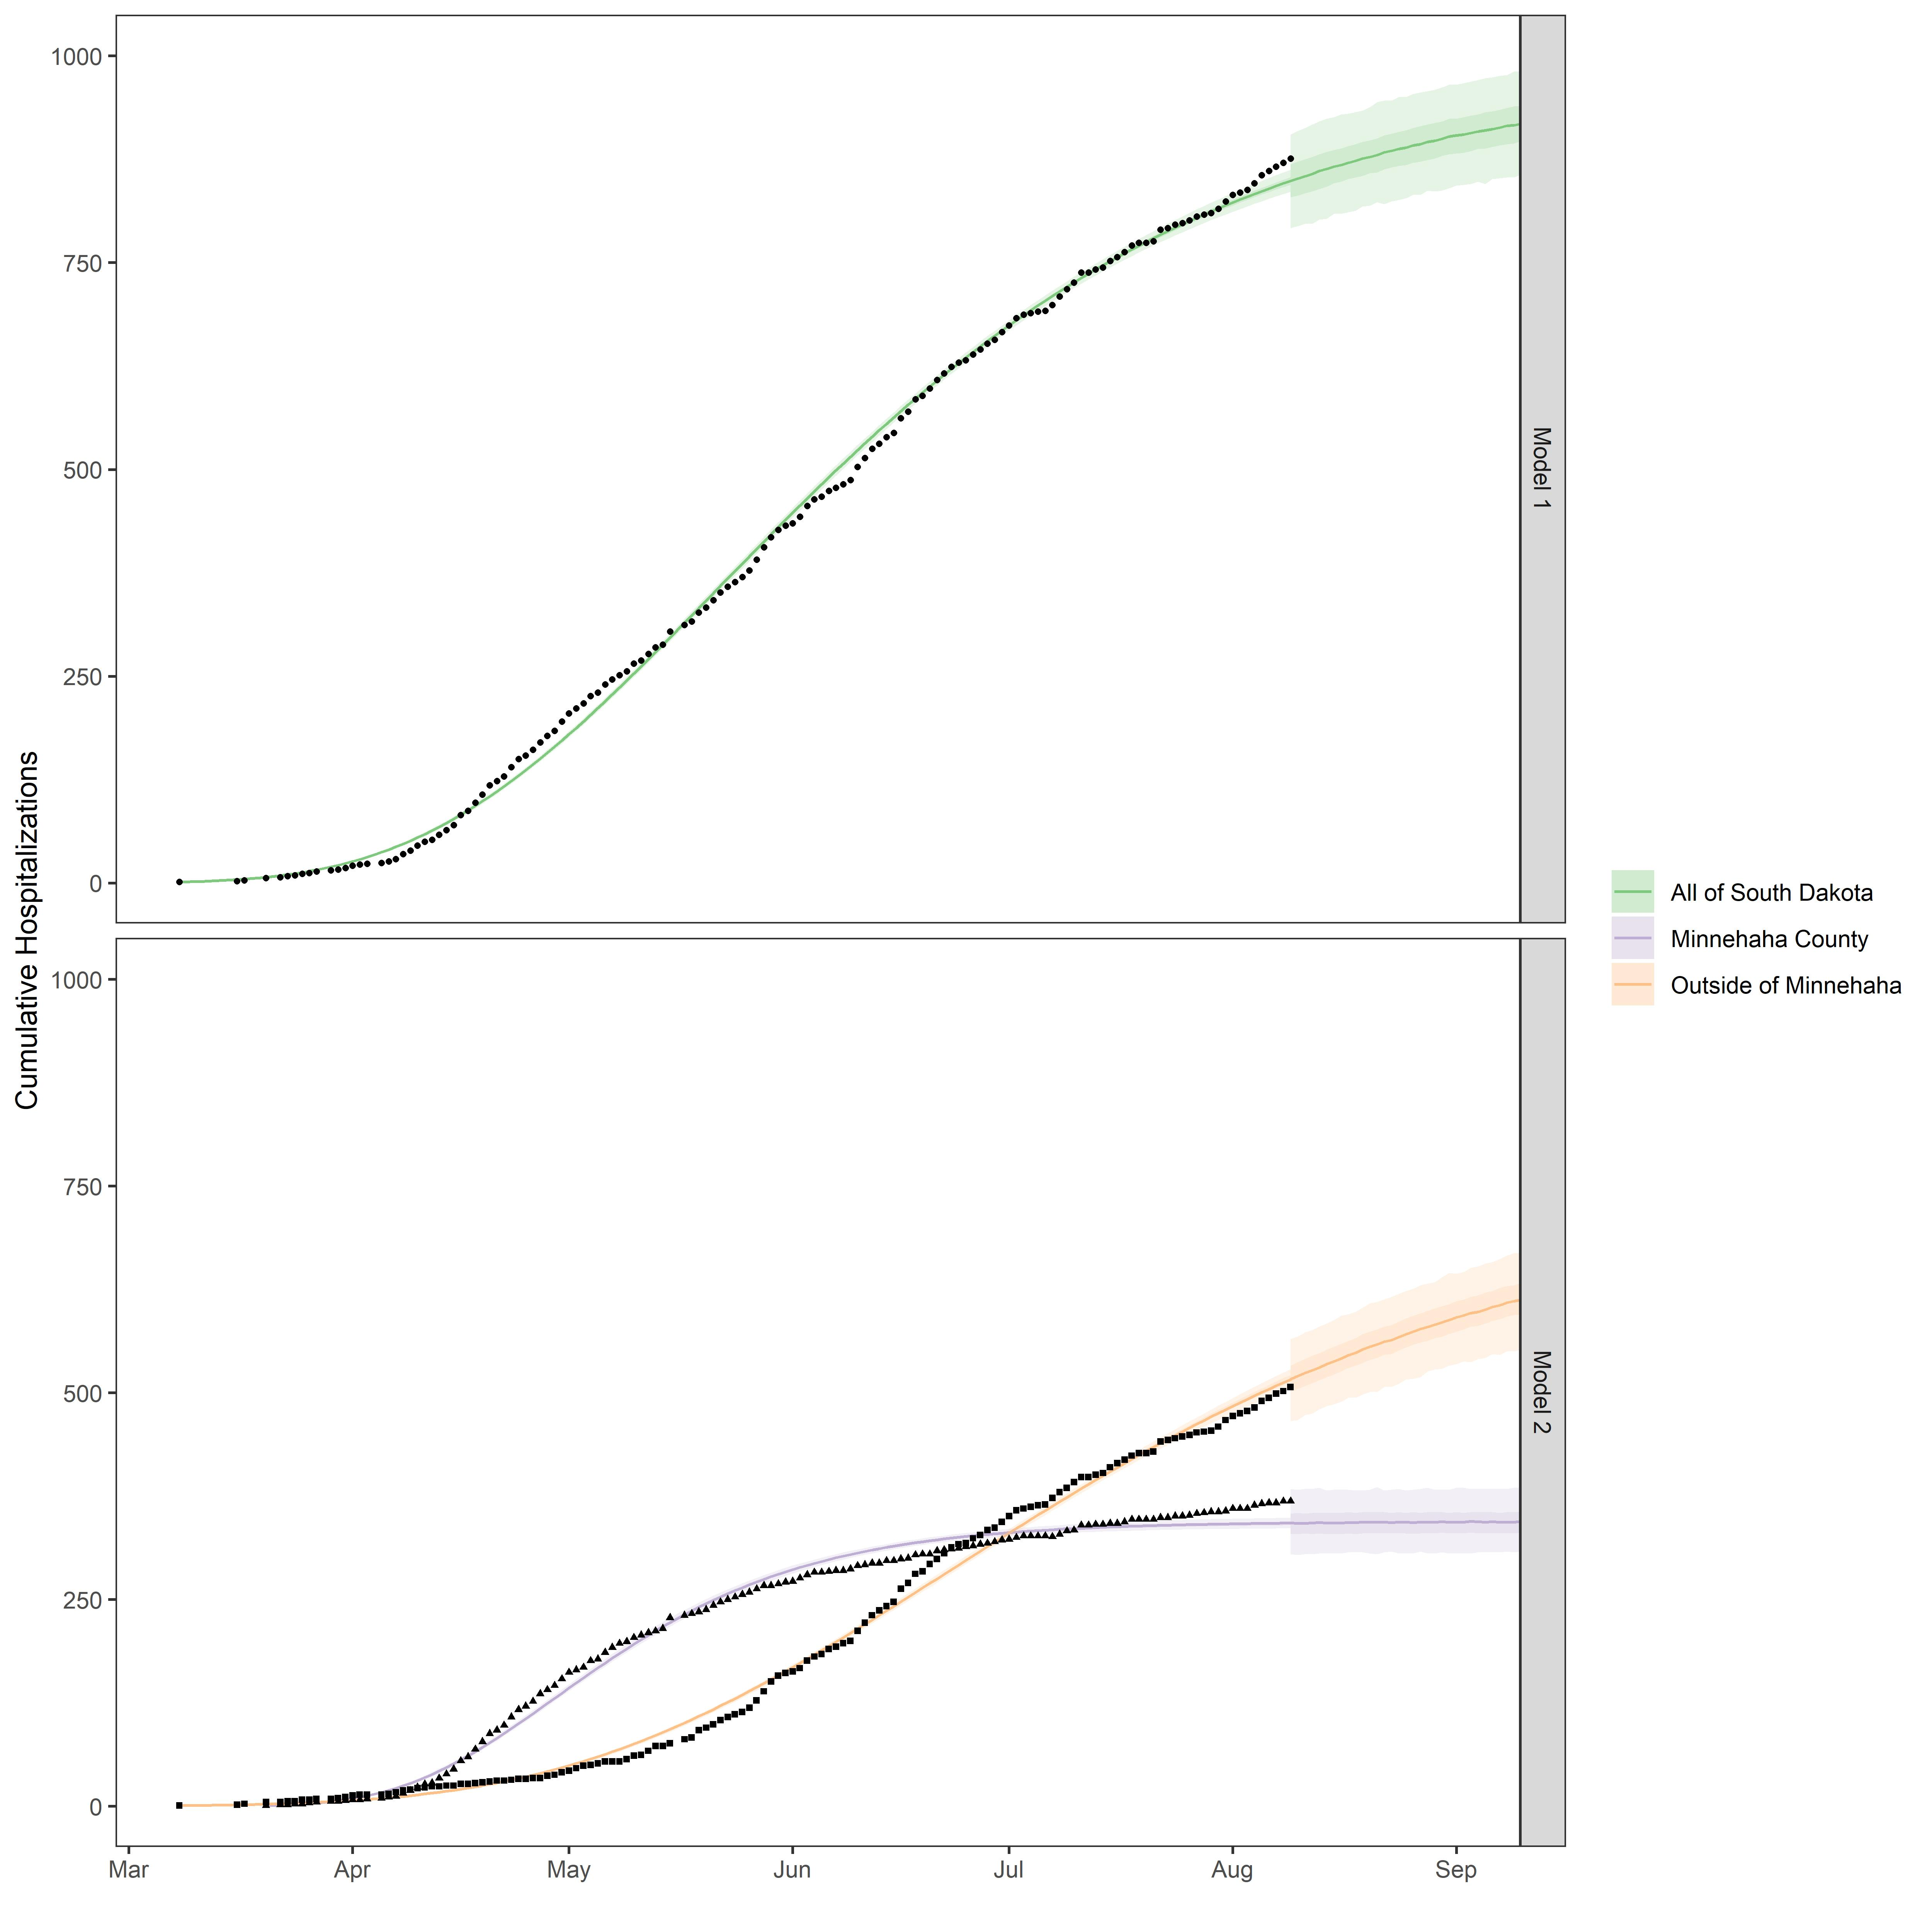
\includegraphics[width=1\linewidth]{C:/Users/Jeff.Wesner/Documents/GitHub/Inquiry_Textbook/images/post_all_plot} \caption{The initial figure. We made this first and then wrote the rest of the paper around it.}\label{fig:unnamed-chunk-3}
\end{figure}
\end{figure}

We spent a lot of time thinking about how to make this figure, because
we used it to guide our writing. A well-made figure is more than just a
visualization. It it also an outline for the paper itself. Here are some
examples, linking that parts of the graph to sections of the written
text.

\textbf{y-axis} The y-axis says ``Cumulative Hospitalizations''. As a
reader, if this figure was all we had seen, we could deduce that the
paper had something to do with hospitalization trends over time. That's
not trivial. There are millions of scientific papers published each year
on a vast array of disciplines (biology, physics, math, sociology, etc).
With just the y-axis here, we now know that this paper is probably in
the field of medicine or public health. It also starts at zero, so we
can surmise that this study is measuring hospitalizations at the
beginning of whatever is causing them.

\textbf{x-axis} The x-axis has abbreviations for seven months, so we can
assume the the predictor variable here is time, and that the duration of
the study is less than one year.

\textbf{key} There are three time trends presented. One of them is for
All of South Dakota. The others are for a county (Minnehaha County) and
everything outside of Minnehaha County.

\textbf{panels} The three time trends are presented across two models
(Model 1 and Model 2). We can't tell much about those models from the
plot alone, but this gives us something to search for in the text.

\textbf{data} The plot appears to show individual data points,
presumably of the number of cumulative hospitalizations on each day. If
we counted them all up, we could know exactly how many data points are
in the analysis.

\textbf{fitted lines} Corresponding to the data are a green, orange, or
purple line with some shading. It is not clear from the plot along what
these represent, and there is an odd-looking change in the shading after
the data points.

Even from this seemingly simple plot, we can glean a lot about the study
before we've ever read a word of the paper. But there is a lot we still
don't know. Who is being hospitalized? What are they being hospitalized
for? What are the two models? What's up with the change in shading after
the data end? As a writer, it is your job to explain these things in the
text.

A well-written paper provides details and context in the written
sections of the paper that make it clear why the study was done (and why
the plot is important to understand). Here are some examples.

\begin{enumerate}
\def\labelenumi{\arabic{enumi})}
\item
  Title: \emph{Forecasting hospitalizations due to COVID-19 in South
  Dakota, USA.} The title sheds a lot of light on the figure. We can
  assume that the y-axis in the figure is probably hospitalizations of
  COVID-19 patients in South Dakota.
\item
  Abstract:
\end{enumerate}

\begin{quote}
\emph{Anticipating the number of hospital beds needed for patients with
COVID-19 remains a challenge. Early efforts to predict hospital bed
needs focused on deriving predictions from SIR models, largely at the
level of countries, provinces, or states\ldots{}}
\end{quote}

The first two sentences of the abstract give further clues as to why the
y-axis in the figure is important to know about. We want to know about
hospitalizations COVID-19 so that we can better anticipate the health
care infrastructure that might be needed. According to the authors,
doing that is a ``challenge'', and other studies have addressed that
challenge in varying ways.

\begin{enumerate}
\def\labelenumi{\arabic{enumi}.}
\setcounter{enumi}{2}
\tightlist
\item
  Introduction:
\end{enumerate}

Here are the first sentences of each paragraph of the introduction.

\begin{quote}
\emph{The novel coronavirus (SARS-CoV-2) was first detected in December
2019 in Wuhan, China and has since spread globally. The disease caused
by SARS-CoV-2\ldots{}}

\emph{Predicting hospitalization needs due to COVID-19 may be
particularly challenging in rural areas. For example, relative}\ldots.

\emph{To our knowledge, there are no published studies that model
hospitalizations due to COVID-19 in rural and low resource settings.}

\emph{Here, we modeled cumulative hospitalizations in an urban
(Minnehaha) versus rural population within South Dakota using a Bayesian
non-linear Weibull function. Because early predictions}\ldots{}
\end{quote}

From skimming just the first sentences of the introduction, we've
discovered that the study is important (according to the authors,
anyway) because it represents hospitalization trends in an urban
(Minnehaha) and rural setting. This helps to explain the \textbf{key} in
the plot above. We shouldn't just take the author's word for it. If we
were skeptical about why this is important to study, then we could find
more justifications in the rest of the introduction. But scanning the
first sentences gives us a quick way to judge the paper's context.

\begin{enumerate}
\def\labelenumi{\arabic{enumi}.}
\setcounter{enumi}{3}
\tightlist
\item
  Methods:
\end{enumerate}

\begin{quote}
\emph{We fit the Weibull function to two sets of data that describe 1)
the cumulative hospitalizations for the state of South Dakota and 2) the
cumulative hospitalizations for subgroups of Minnehaha County and the
rest of South Dakota.}
\end{quote}

This sentence from the methods resolves the two \textbf{panels}. Now we
know that the authors fit the data in two ways, and that model 2 appears
to use data that are subgroups of model 1.

\begin{enumerate}
\def\labelenumi{\arabic{enumi}.}
\setcounter{enumi}{4}
\tightlist
\item
  Results:
\end{enumerate}

\begin{quote}
At the state level, model 1 predicted a total of 876 hospitalizations
(median) in South Dakota (90\% CrI: 834-926, Table 2). The inflection
point was predicted at 37 days after the first hospitalization,
suggesting that the peak rate of hospitalizations occurred around April
20, 2020 (Table 2). In contrast, the model with group-level effects
clearly showed that hospitalizations trends differed in Minnehaha County
verses the rest of South Dakota\ldots{}
\end{quote}

The results section here is three paragraphs long, and we've only pasted
a few sentences from it. In the results, we can expect to find
quantitative summaries that describe what we see in the graph.

\begin{enumerate}
\def\labelenumi{\arabic{enumi}.}
\setcounter{enumi}{5}
\tightlist
\item
  Discussion:
\end{enumerate}

\begin{quote}
The most important result of this study is that modeling trends
separately in urban versus rural parts of a state population reveal
different projections of cumulative hospitalizations than if modeled
only using state-level data. In particular, the model\ldots{}
\end{quote}

The discussion continues to provide context for the details in the rest
of the paper. Now we can see what the author's think is the most
important result, and how the patterns in the plot reinforce that
result. We don't have to agree with this. There are other parts to the
paper and maybe we think those are more important\ldots or that the
paper is not really interesting at all. That is all fine. The main point
is that we are able to judge the work based on clearly written text.

This method - \emph{Figures First} - is helpful in two ways. 1) It helps
us to organize our writing, and 2) It helps us to quickly read and
understand other scientific papers. Try it out!

\end{document}
